% LaTeX Template for Project Report, Version 2.0
% (Abstracted from a Major Project Report at CSED, NIT Calicut but can be
% modified easily to use for other reports also.)
%
% Released under Creative Commons Attribution license (CC-BY)
% Info: http://creativecommons.org/licenses/by/3.0/
%
% Created by: Kartik Singhal
% BTech CSE Batch of 2009-13
% NIT Calicut
% Contact Info: kartiksinghal@gmail.com
%
% It is advisable to learn the basics of LaTeX before using this template.
% A good resource to start with is http://en.wikibooks.org/wiki/LaTeX/
%
% All template fields are marked with a pair of angular brackets e.g. <title here>
% except for the ones defining citation names in ref.tex.
%
% Empty space after chapter/section/subsection titles can be used to insert text.
%
% Just compile this file using pdflatex after making all required changes.

\documentclass[12pt,a4paper]{report}
\usepackage[pdftex]{graphicx} %for embedding images
\usepackage{url} %for proper url entries
\usepackage{booktabs}
\usepackage[colorinlistoftodos]{todonotes}
\usepackage[bookmarks, colorlinks=false, pdfborder={0 0 0}, pdftitle={<MEng Individual Project Interim Report>}, pdfauthor={<Yangfan Zhang>}, pdfsubject={<Computing>}, pdfkeywords={<TFL, Bus Arrival Times, Delay>}]{hyperref} %for creating links in the pdf version and other additional pdf attributes, no effect on the printed document
%\usepackage[final]{pdfpages} %for embedding another pdf, remove if not required

\begin{document}
\renewcommand\bibname{References} %Renames "Bibliography" to "References" on ref page

%include other pages
\begin{titlepage}

\newcommand{\HRule}{\rule{\linewidth}{0.5mm}} % Defines a new command for the horizontal lines, change thickness here

\center % Center everything on the page
 
%----------------------------------------------------------------------------------------
%	HEADING SECTIONS
%----------------------------------------------------------------------------------------

\textsc{\LARGE Imperial College London}\\[1.5cm] % Name of your university/college
\textsc{\Large Department of Computing}\\[0.5cm] % Major heading such as course name
\textsc{\large MEng Individual Project Interim Report}\\[0.5cm] % Minor heading such as course title

%----------------------------------------------------------------------------------------
%	TITLE SECTION
%----------------------------------------------------------------------------------------

\HRule \\[0.4cm]
{ \huge \bfseries Active Delay Warning Transport App}\\[0.4cm] % Title of your document
\HRule \\[1.5cm]
 
%----------------------------------------------------------------------------------------
%	AUTHOR SECTION
%----------------------------------------------------------------------------------------

\begin{minipage}{0.4\textwidth}
\begin{flushleft} \large
\emph{Author:}\\
Yangfan \textsc{Zhang} % Your name
\end{flushleft}
\end{minipage}
~
\begin{minipage}{0.4\textwidth}
\begin{flushright} \large
\emph{Supervisor:} \\
Dr. Peter \textsc{McBrien} % Supervisor's Name
\end{flushright}
\end{minipage}\\[4cm]
% If you don't want a supervisor, uncomment the two lines below and remove the section above
%\Large \emph{Author:}\\
%John \textsc{Smith}\\[3cm] % Your name

%----------------------------------------------------------------------------------------
%	DATE SECTION
%----------------------------------------------------------------------------------------

{\large \today}\\[3cm] % Date, change the \today to a set date if you want to be precise

%----------------------------------------------------------------------------------------
%	LOGO SECTION
%----------------------------------------------------------------------------------------

%\includegraphics{Logo}\\[1cm] % Include a department/university logo - this will require the graphicx package
 
%----------------------------------------------------------------------------------------

\vfill % Fill the rest of the page with whitespace

\end{titlepage}
%!TEX root = report.tex
\vspace{2in}
\begin{abstract}
\todo[inline]{abstract}
<Abstract here>
The abstract is a very brief summary of the report's contents. It should be about half a page long. Somebody unfamiliar with your project should have a good idea of what it's about having read the abstract alone and will know whether it will be of interest to them. Note that the abstract is a summary of the entire project including its conclusions. A common mistake is to provide only introductory elements in the abstract without saying what has been achieved.

\end{abstract}
%!TEX root = report.tex
\cleardoublepage
%\pagebreak
\phantomsection
\addcontentsline{toc}{chapter}{Acknowledgements}
\chapter*{Acknowledgments}
\vspace{1.0in}
<Acknowledgements here>
Peter McBrien, Susan
\\
\\
\\
\\
<Name here> \\
\\
\\
<Month and Year here>\\
{National Institute of Technology Calicut}\\
\newpage


\pagenumbering{roman} %numbering before main content starts
\tableofcontents
% \listoffigures

\listoftodos

\newpage
\pagenumbering{arabic} %reset numbering to normal for the main content

%\input{./prob-definition.tex} %objective changed to problem definition
%!TEX root = report.tex
\chapter{Introduction}

The London bus network carries 2.4 billion passengers a year, more than the rest of England combined \cite{tfl_annual_report_13/14}.

\par The bus arrival times published by Transport for London (TfL) are currently widely available on digital live bus arrivals signs at more than 2,500 bus stops \cite{live_bus_arrivals}. Passengers can also check this information by sending a text message with the bus stop code, as well as doing a quick search online or on mobile applications.

\todo[inline]{Passengers chose travel mode based on travel time and convenience. Find evidence for this assumption. How do people choose travel mode / whether to take bus? }

\todo[inline]{Scenario, a passenger chose to take a bus, then only realises delay at the end of the journey. Would have chosen another mode of travel should he know of the delay earlier.}

\par Passengers rely on the bus arrival times to plan their journey, by factoring in the waiting time when choosing the buses to take. Current London journey planning software takes the journey start time, start location, and destination as input, and recommends routes consisting of a variety of travel mode, with an estimate travel time for each suggested journey. Such popular planners include Google maps \cite{google_maps}, Citymapper \cite{citymapper} and Transport for London Journey Planner \cite{tfl_journey_planner}.

\par However, the accuracy of the bus arrival times published is affected by many external factors. For example, when there is heavy traffic, the buses are likely to be delayed by a difference significant enough for a change in passengers' route picking. Yet, this delay information is not reflected in the arrival time data or the estimated journey time early enough for the passengers to make a decision to choose an alternate route. As a result, passengers waste time waiting for buses that come much later than expected, or chosing to board a bus that takes far longer than the estimated journey time. Although the average bus delay is 1 minute, there was a 16.6 chance of waiting for more than 10 minutes \cite{buses_performance_data}.

\par This can be avoided if passengers are informed of the delays in bus arrival times in advance. Such delays can predicted by analysing the historical delays. This is achieved by collecting data from the Transport for London live bus arrivals API stream feed\cite{live_bus_arrivals}, and estimate the average journey time required between two locations on a given time of the day. Next, a bus arrival time table with delays during various time windows over a week can be crafted and fine tuned incrementally. We compared the travel times in this timetable with the official travel times published by the Transport of London Open Data to find out the delays in bus arrival times. %literature survey included in this
%!TEX root = report.tex
\chapter{Background}

\section{London Bus Network}

\par The bus network in London is one of the largest and most accessible in the world. It is carrying a staggering number of passengers, with more than 2.4 billion journeys in 2013/14, which was more than any year since 1959 \cite{tfl_annual_report_13/14}.

\par On an average day between 2005 and 2010, about 14\% of the trips made by London residents were by bus \cite{tfl_ltds}. They spent on average 14 minutes per day on these bus trips.

\par There are currently 19,345 bus stops, and 680 routes served by 8,765 buses daily in London\cite{bus_stop_locations_routes}.

\todo[inline, color=purple]{produce graph for this, number of stops, routes and buses}
% number of people that use apps to plan journey or pick the bus to take

\subsection{Bus Network Performance}

\par TfL published the following figures in the second quarter 2014/2015 buses performance data \cite{buses_performance_report}.

\par For the high frequency services, the average scheduled wait was 4.86 minutes, the average excess wait was 0.94 minutes, and the average actual wait was 5.80 minutes. While passengers could expect the buses to come within 10 minutes 83.4\% of the time, there was 15.1\% chance of waiting for 10-20 minutes, 1.3\% chance of waiting for 20-30 minutes, and 0.2\% chance of waiting for more than 30 minutes.

\par For the low frequency services, 87\% of the buses services were on time, and 11.4\% were 5-15 minutes late.

\par For the night buses, 84.5\% of the services were on time. The average excess wait was 0.68 minutes.

\todo[inline, color=purple]{produce graph here}

\par The bus arrivals might be affected by traffic congestion, staff availability, engineering problems, or mechanical breakdown \cite{buses_performance_data}.

\section{Buses Status Updates}
\par To inform passengers of the bus service disruptions or diversions, \acrshort{tfl} provides a bus status updates service online \cite{tfl_buses_status_updates}. Passengers can retrieve relevant bus service status for a given bus stop or route (Figure \ref{fig:tfl_status_update}).

\begin{figure}
\centering
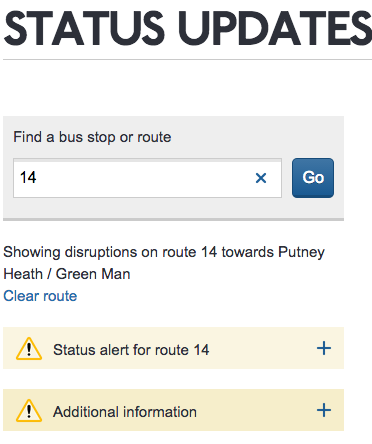
\includegraphics[width=0.5\textwidth]{figures/tfl_status_update.png}
\caption{\label{fig:tfl_status_update} Tfl Buses Status Update Service}
\end{figure}

\par The textual information include service disruptions, diversion, suspensions, and delays due to heavy traffic.

\par While this service informs passengers of current abnormal bus schedules, it requires passengers to visit the site to check for specific information, and does not provide an estimation on the travel time under the special conditions.

\par \acrshort{tfl} also publishes live status news and updates on Twitter \cite{tfl_bus_alerts_twitter}, but it is not easily searchable by passengers to check specific information relevant to their journeys.

\par Additionally, many current popular journey planners such as Google Maps\cite{google_maps}, Citymapper London\cite{citymapper}, and \acrshort{tfl} Journey Planner incorporate the bus delay information in the suggested journeys as a textual alert. These apps do not recompute the estimated journey time for passengers to make an informed decision.

\par As a result, the lack of data service on bus delay predictions and travel times



. This presents a significant barrier to bus passengers who wish to plan their bus journeys for specific appointments.

\section{Choice of Travel Mode}
\todo[inline]{Does the arrival time / delay affect people's choice of travel mode? What are the purposes of commute? Work, travel, leisure, appointments?}

%!TEX root = report.tex
\section{Transport for London Open Data}
\acrshort{tfl} provides data to quantify the delays in bus journey time. We collected the necessary data from the Live Bus Arrivals \acrshort{api}, Bus Stop Locations and Routes, and Journey Planner Bus Timetables. The Live Bus Arrivals \acrshort{api} enables a query to receive a bespoke response, depending on the parameters supplied. Bus Stop Locations and Routes come as static data files which rarely change. Journey Planner Bus Timetables are feeds that refresh at regular intervals.

%!TEX root = report.tex
\subsection{Live Bus Arrivals API Stream}
\par The Live Bus Arrivals API Stream provides the predicted time until a bus is expected to arrive at a stop. These predictions are available for the next 30 minutes at any point in time. For example, at 9am, the stream will provide predicted bus arrivals up to 9.30am on the same day. This data is refreshed every 30 seconds \cite{live_bus_api_documentation}.

\par The base URL is \url{http://countdown.api.tfl.gov.uk/interfaces/ura/stream_V1}. In order to collect bus arrival data for analysis, we supplied the following parameters which specify the fields returned by the \acrshort{api}.



%!TEX root = report.tex
\subsection{Bus Stop Locations and Routes}
\par The TFL Open Data provides network information on the location of all bus stops in London, and the sequence of bus stops in every bus route.

\par This data is in the comma-separated values (CSV) format. We imported the bus sequences into the delay\_bus\_sequences table (Table \ref{table:delay_bus_sequences})

\begin{table}
\centering
\begin{tabular}{@{}llr@{}} \toprule
Column Name & Type & Comments\\ \midrule
id(Primary Key) & int(11)  & Auto Increment\\
route & varchar(64) &  The route name\\
run & int(11) & The route direction\\
sequence & int(11) & The sequence of the bus stop in the route\\
stop\_code\_lbsl & varchar(64) & The internal bus stop identifier\\
bus\_stop\_code & varcher(64) & The public code for the bus stop\\
naptan\_atco & varchar(64) & The national identifier of the bus stop\\
stop\_name & varchar(64) & The name of the bus stop\\ \bottomrule
\end{tabular}
\caption{delay\_bus\_sequences Table Schema}
\label{table:delay_bus_sequences}
\end{table}
 \todo[inline, color=cyan]{Question: Can I skip some columns of the table schema, as those columns have not been used in the project, but just storing as reference for now?}
\par Additionally, we extracted information on all pairs of neighbouring bus stops and the routes that serve between them. We save this information in the delay\_neighbours table (Table \ref{table:delay_neighbours}). See sample data in Table \ref{table:sample_neighbours_view}.

\begin{table}
\centering
\begin{tabular}{@{}llr@{}} \toprule
Column Name & Type & Comments\\ \midrule
id(Primary Key) & int(11)  & Auto Increment\\
route & varchar(64) & The bus route \\
start\_stop & varchar(64) & The stop\_code\_lbsl for the start stop\\
end\_stop & varcher(64) & The stop\_code\_lbsl for the end stop\\ \bottomrule
\end{tabular}
\caption{delay\_neighbours Table Schema}
\label{table:delay_neighbours}
\end{table}

\begin{table}
\centering
\begin{tabular}{@{}llrr@{}} \toprule
id & route & start\_stop & end\_stop \\ \midrule
18433 & 30 & 10002 & 11469 \\
44878 & N19 & 10002 & 11469 \\
47128 & N41 & 10002 & 29772 \\
8653 & 19 & 10002 & 11469 \\ \bottomrule
\end{tabular}
\caption{Sample data in delay\_neighbours Table}
\label{table:sample_neighbours_view}
\end{table}

\subsubsection{Finding the average travel time between neighbouring stops}
\todo[inline] {update this part}
\par To experiment with the queries, we selected one pair of the neighbouring stops (10002, 11469), and listed the time required to travel from stop 10002 to stop 11469 by finding the difference in arrival times for each journey. Sample entries of this list is shown in Figure \ref{fig:journey_time_10002}.

\begin{figure}
\centering
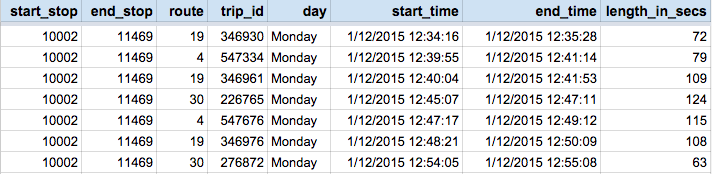
\includegraphics[width=0.7\textwidth]{figures/journey_time_10002.png}
\caption{\label{fig:journey_time_10002} List of journey time from stop 10002 to stop 11469}
\end{figure}


\par We then calculated the average journey time required to travel from 10002 to 11469 for each hour in each week of the day. This information is stored as a timetable, which would be used for further analysis.

Figure\ref{fig:timetable_10002} shows the timetable generated. Each cell indicates the average journey time required to travel from stop 10002 to stop 11469 at a give hour of a give week of day. The \textbf{NULL} values are due to a current databases performance issue. This will be resolved later.

\begin{figure}
\centering
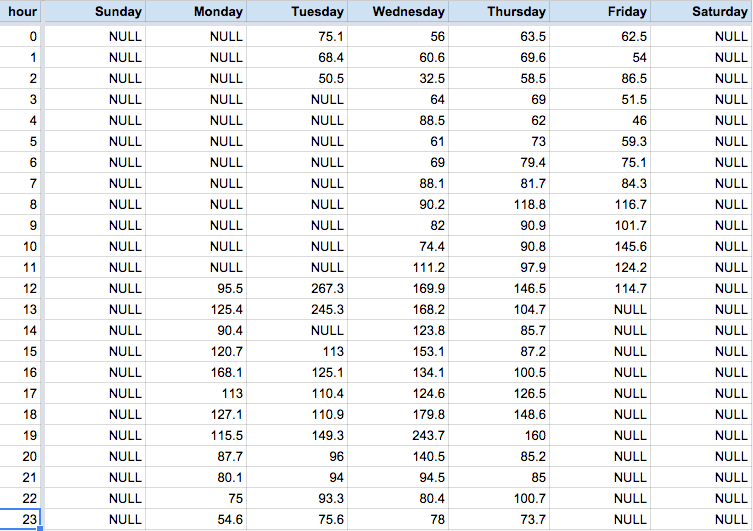
\includegraphics[width=0.9\textwidth]{figures/timetable_10002.png}
\caption{\label{fig:timetable_10002} Average journey time in seconds from stop 10002 to stop 11469 for each hour of each day of week}
\end{figure}

\par We plan to construct a timetable this way for each pair of the neighbouring bus stop.
%!TEX root = report.tex
\subsection{Journey Planner Bus Timetables}
The Journey Planner Bus Timetables \cite{open_data_feeds_description} contains information on official bus schedules including stops, routes, departures times, departure frequencies, operational notes, as well as the days on which the services run.

The timetables uses the \acrfull{xml} \cite{xml} format, with the schema defined in \gls{transxchange} \cite{transxchange}, the UK nationwide standard for exchanging bus schedules and related data. For this project, we used the General schema version 2.1\cite{transxchange_downloads_and_schema}\cite{transxchange_schema_2.1_xsd}, the latest available version for download. Each \acrshort{xml} file contains the bus timetables for one route. Figure \ref{fig:xml_components} shows the overview of a timetable \acrshort{xml} file.

\begin{figure}
\centering
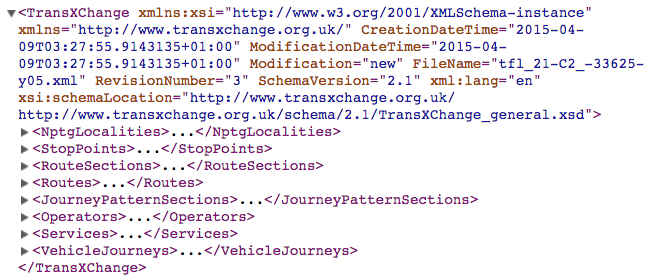
\includegraphics[width=1\textwidth]{figures/xml_components.png}
\caption{\label{fig:xml_components} TfL Journey Planner Timetables Sample XML Overview}
\end{figure}

\subsubsection{Data Structure}
The \gls{transxchange} timetable model has the following seven basic concepts\cite{transxchange_schema_guide}:

\begin{enumerate}
  \item \texttt{Service} contains one or more \texttt{JourneyPattern} elements and one or more \texttt{VehicleJourney} elements. This is the basic concept that brings together the information about a registered bus service.
  \item \texttt{Registration} specifies the registration details for a service.
  \item \texttt{Operator} indicates the entity who runs the service.
  \item \texttt{Route} describes the physical path taken by buses on the service as an ordered list of \texttt{StopPoints}.
  \item \texttt{StopPoint} contains reusable declarations of the stops used by the routes and journey patterns of the schedule. All StopPointRef instances elsewhere in a document are resolved against the contents of the StopPoints element. All stops are defined as being \gls{naptan} points.
  \item \texttt{JourneyPattern} specifies an ordered list of links between the \texttt{StopPoints}, giving the \emph{relative travel times} between each pair of neighbouring stops.
  \item \texttt{VehicleJourney} specifies the individual scheduled journey \emph{at a specific absolute time}.
\end{enumerate}

These elements give a complete official bus schedule for each route with the departure time for each bus journey, the relative bus travel time between stops, and the days on which the service operates on. We extracted the official bus timetables from these \acrshort{xml} files, as discussed in Section \ref{sec: official_tfl_timetable}.

%!TEX root = report.tex
\subsection{iBus System}
The actual arrival time of buses on a route at any given bus stop for the selected day are made available by the London Buses iBus system.

Currently, the routes were selected as the first of the New Routemaster (New Bus for London). Data will be published once a week \cite{buses_performance_data}.

This data is stored in comma-separated values (CSV) format. There are two potential uses for this data.
\begin{itemize}
	\item We can integrate it into the arrivals table to improve the precision of the arrivals data. Since the current entries in the arrivals table contain estimated bus arrival times, the integrated of the iBus data which contains real bus arrival times will likely boost the precision of the data in arrival table.
	\item We can compare the predicted delays with the iBus data for performance evaluation.
\end{itemize}

\section{Additional Background Materials}
Here's a list of the potential points to be covered in the final report.

\begin{itemize}
	\item Geocoding data
    \item Possible analysis methodologies such as regression
    \item Literature review on similar research done in other areas of the world
\end{itemize}

\todo[inline]{document a service that other developers can use, with demo app to show the features}
\todo[inline]{background on other apps}
\todo[inline]{document the DB}


% \section{Other Available Data}
% \subsection{Greater London Data}
% \subsection{Geocoding}

% \section{Analysis Methodologies}
% % \todo[inline]{I am not really sure what methods to use for analysis}
% \subsection{Regression}
% \subsection{Statistical Analysis}

% \section{Literature}
% \subsection{TFL Journey Planner}
% The website’s Journey Planner and homepage
% status board have also been redesigned and
% integrated so customers planning their trip can
% see immediately if their route is likely to be
% affected by upgrade work or other disruptions.
% The Journey Planner will now automatically
% generate cycling and walking routes, giving
% people a wider range of options for their journey \cite{tfl_annual_report_13/14}

% \subsection{Google Maps}
% \subsection{City Mapper London}


%!TEX root = report.tex
\subsection{Summary on Available Data}
\par While there is sufficient data on London bus network, official bus timetables, and live arrival times, there is no data service offering real-time predictions on bus delays.

\par \acrshort{tfl} releases information on service disruption, yet this is not incorporated


There is also a status updates service for passengers to check disruptions on the given bus stop or route.


%!TEX root = report.tex
\section{Current Travel Applications}

\begin{figure}
\centering
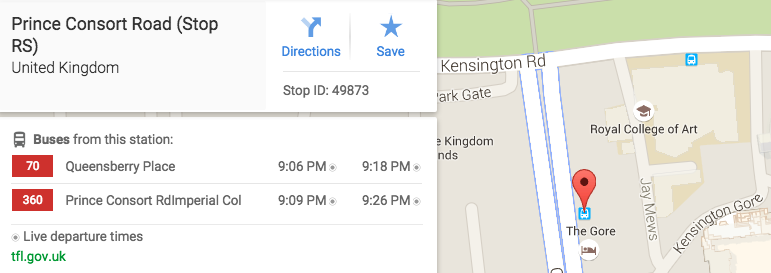
\includegraphics[width=1\textwidth]{figures/google_maps_tfl_data.png}
\caption{\label{fig:google_maps_tfl_data} Google Maps Using TfL Bus Arrival Data}
\end{figure}

Over 5,000 developers have registered for the open data\cite{open_data}, and around 200 travel apps are powered by it \cite{tfl_annual_report_13/14}. The most popular travel applications include \acrshort{tfl} Journey Planner, Google Maps (Figure \ref{fig:google_maps_tfl_data}), and Citymapper London. Given the departing location, destination, as well as departure time, these applications can provide suggested routes and travel times. Users can further customise their desired journey by specifying the desired walking distance, and accessibility requirements. Moreover, the \acrshort{tfl} Journey Planner and homepage
status board were redesigned and integrated so customers planning their trip can see immediately if their route is likely to be affected by upgrade work or other disruptions \cite{tfl_annual_report_13/14}, with a textual warning message shown.

\par However, currently, there are no applications that give predictions on travel times and warnings on potential delays. The estimated travel time shown in apps is extracted from the \acrshort{tfl} Journey Planner Bus Timetables. This information does not capture the real time delays according to instant traffic conditions.

%!TEX root = report.tex
\chapter{Concept Design}
\section{Objectives}
\par We aim to improve the prediction of bus travel time downstream from location of last observation in mixed traffic operations. We achieve this by providing an API data service of bus travel time predictions, and a demonstrative web application to show case the use of such a data service.

\section{Bus Travel Times}
\par The bus travel time between 2 neighbouring stops depends on many unpredictable external factors. These include weather conditions, passenger flow, temporary lane closures, as well as the time of the bus trip. Predicting bus travel times by discovering and analysing these contributing factors is complicated.

\par We decided to bypass looking at these factors, and examine the historical and current bus travel times instead. We assumed that for a specific short time frame, the external factors remain largely unchanged. In this case, the bus travel time between the given 2 neighbouring stops is similar to the previous trips performed in the same time frame.

\par For bus travel time between every pair of neighbouring stop at each hour of the day, we provide estimations for the following:
\begin{itemize}
  \item \textbf{Reference Timtable} How long does TfL says it take?
  \item \textbf{Current Timetable} How long does it currently take?
  \item \textbf{Historical Timetable} How long does it usually take?
\end{itemize}

\par Since the reference timetable shows the typical bus travel time, the historical timetable should converge to the reference timetable over time.

\par The current timetable shows the most relevant bus travel time at the observation point, a significant increase in travel time compared to the historical or refernece timetables would indicate a bus delay.

\subsection{Reference Timetable}
\par We extracted the average bus travel time between every pair of neighbouring stops for every route during every hour of the day for every day of the week from the \acrshort{tfl} Journey Planner Bus Timetables. This is discussed in Section \ref{sec: official_tfl_timetable}.

\subsection{Current Timetable}
\par We collect the live bus arrival times for the past 1 hour, and store the final bus arrival times for each bus at each stop. We then find out the travel time of each bus between every pair of neighbouring stops for the given hour. Next, we calculate the average travel time between each pair of neighbouring bus stops. This serves as a prediction for how long the bus currently takes to travel between two neighbouring stops. See implementation details in Section \ref{sec:current_timetable_generation}.

\subsection{Historical Timetable}
\par We store the current timetable generated at each hour, and group them by the hour of the day for the same day of the week. We then calculate the average bus travel time between each pair of neighbouring stops for each hour of the day in each day of the week. For example, the average bus travel time between stop A and stop B for 3pm on Wednesday is the average travel time for all the bus trips between these two stops between 2pm to 3pm in the past Wednesdays. More details cound be found in Section \ref{sec:historical_timetable}.

\section{Contributions}
\par We provided the above mentioned three timetables as an API data service (Chapter \ref{ch:data_service}) and designed a demostrative mbile application that warns users of current bus delays from a given bus stop (Chapter \ref{ch:mobile_app}).


\section{Architecture Design}
\begin{itemize}
\item Used Django Framework to build the backend that retrieves data from a MySQL database.

\item Used AngularJS with Twitter Bootstrap for frontend development
\end{itemize}
\missingfigure{graph to show the overall structure}






%!TEX root = report.tex
\chapter{Data Collection and Generation}
\label{ch:data_generation}
\section{Overview}

\todo[inline]{UML diagrams}

\section{Development Environment}
\subsection{Virtual Machine}

\subsection{MySQL Databases}
\par We chose to use MySQL to store the data for the following benefits it offers:

\begin{itemize}
  \item \textbf{User Interface} MySQL has convenient database management tools such as phpMyAdmin\cite{phpmyadmin} and Sequel Pro\cite{sequel_pro} for easy data browsing.
  \item \textbf{Scalability} MySQL can handle memory heavy computation efficiently, given the correct configuration.
\end{itemize}

\section{Generating Historical Timetable}
\begin{itemize}
  \item data collection
  \item data storing
  \item data processing
  \item DB optimisation
  \item python scripts and SQLs
  \item resulting table name and schema
\end{itemize}

\subsection{Collecting Bus Arrival Times}
\label{sec:collecting_arrival_times}

\par We collect bus arrival data for analysis from the live bus arrivals API. The base URL used in this project was \url{http://countdown.api.tfl.gov.uk/interfaces/ura/stream_V1}.

\par We supplied the following parameters which specify the fields returned by the \acrshort{api}.

\begin{itemize}
  \item \textit{StopID} This is the alphanumeric identifier of a bus stop. It is also known as stop\_code\_lbsl.
  \item \textit{LineName} This is the route number that is displayed on the front of the bus on any publicity advertising the route.
  \item \textit{VehicleID} The unique identifier of the vehicle.
  \item \textit{TripID} The identifer of the specific trip that the prediction is for.
  \item \textit{EstimatedTime} This is the predicted time of arrival for the vehicle at a specific stop.
  \item \textit{ExpireTime} This is the time at which the corresponding prediction is no longer valid and should stop being displayed.
\end{itemize}

\par The resulting query URL is \sloppy \url{http://countdown.api.tfl.gov.uk/interfaces/ura/stream_V1?ReturnList=StopID,LineName,VehicleID,TripID,EstimatedTime,ExpireTime}.

\par Each data entry contains an estimated arrival time for each bus journey at a given bus stop. This estimated arrival time is stored in the database via an UPDATE statement, which ensures that only the latest estimated arrival times per journey per bus stop are stored. To avoid having data being overwritten, only the entries that have been changed in the recent 10 minutes can be updated. This has been achieved through running a daemon process written in python on a virtual host. Table \ref{table:delay_arrivals_schema} shows the schema for arrivals table.

\begin{table}
\centering
\begin{tabular}{@{}llr@{}} \toprule
Column Name & Type & Default \\ \midrule
id(Primary) & int(11) & Auto Increment \\
stop\_code\_lbsl & varchar(64) &  \\
route & varchar(64) &  \\
vehicle\_id & varchar(64) & \\
trip\_id & varchar(64) & \\
arrival\_date & date &  \\
arrival\_time & timestamp & NULL \\
expire\_time & timestamp & NULL \\
recorded\_time & timestamp & Current Timestamp \\ \bottomrule
\end{tabular}
\caption{delay\_arrivals Table Schema}
\label{table:delay_arrivals_schema}
\end{table}

\subsubsection{Assumption}
We assume that the actual bus arrival time is the midpoint between the last estimated arrival time, and the system time when the clear signal (\textit{ExpireTime} = 0) is received.

\subsection{Neighbouring Stops}
\label{sec:bus_stop_locations_routes}
We imported the bus sequences into the delay\_bus\_sequences table (Table \ref{table:delay_bus_sequences})

\begin{table}
\centering
\begin{tabular}{@{}llr@{}} \toprule
Column Name & Type & Comments\\ \midrule
id(Primary Key) & int(11)  & Auto Increment\\
route & varchar(64) &  The route name\\
run & int(11) & The route direction\\
sequence & int(11) & The sequence of the bus stop in the route\\
stop\_code\_lbsl & varchar(64) & The internal bus stop identifier\\
bus\_stop\_code & varcher(64) & The public code for the bus stop\\
naptan\_atco & varchar(64) & The national identifier of the bus stop\\
stop\_name & varchar(64) & The name of the bus stop\\ \bottomrule
\end{tabular}
\caption{delay\_bus\_sequences Table Schema}
\label{table:delay_bus_sequences}
\end{table}
 \todo[inline, color=cyan]{Question: Can I skip some columns of the table schema, as those columns have not been used in the project, but just storing as reference for now?}
\par Additionally, we extracted information on all pairs of neighbouring bus stops and the routes that serve between them. We save this information in the delay\_neighbours table (Table \ref{table:delay_neighbours}). See sample data in Table \ref{table:sample_neighbours_view}.

\begin{table}
\centering
\begin{tabular}{@{}llr@{}} \toprule
Column Name & Type & Comments\\ \midrule
id(Primary Key) & int(11)  & Auto Increment\\
route & varchar(64) & The bus route \\
start\_stop & varchar(64) & The stop\_code\_lbsl for the start stop\\
end\_stop & varcher(64) & The stop\_code\_lbsl for the end stop\\ \bottomrule
\end{tabular}
\caption{delay\_neighbours Table Schema}
\label{table:delay_neighbours}
\end{table}

\begin{table}
\centering
\begin{tabular}{@{}llrr@{}} \toprule
id & route & start\_stop & end\_stop \\ \midrule
18433 & 30 & 10002 & 11469 \\
44878 & N19 & 10002 & 11469 \\
47128 & N41 & 10002 & 29772 \\
8653 & 19 & 10002 & 11469 \\ \bottomrule
\end{tabular}
\caption{Sample data in delay\_neighbours Table}
\label{table:sample_neighbours_view}
\end{table}

\subsection{Finding the average travel time between neighbouring stops}
\todo[inline] {update this part}
\par To experiment with the queries, we selected one pair of the neighbouring stops (10002, 11469), and listed the time required to travel from stop 10002 to stop 11469 by finding the difference in arrival times for each journey. Sample entries of this list is shown in Figure \ref{fig:journey_time_10002}.

\begin{figure}
\centering
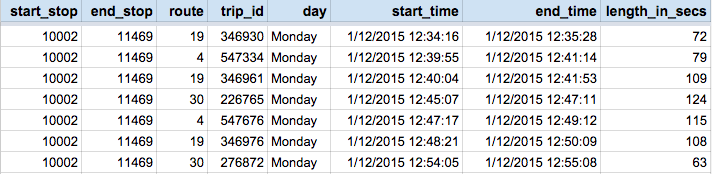
\includegraphics[width=0.7\textwidth]{figures/journey_time_10002.png}
\caption{\label{fig:journey_time_10002} List of journey time from stop 10002 to stop 11469}
\end{figure}

\par We then calculated the average journey time required to travel from 10002 to 11469 for each hour in each week of the day. This information is stored as a timetable, which would be used for further analysis.

\par Figure\ref{fig:timetable_10002} shows the timetable generated. Each cell indicates the average journey time required to travel from stop 10002 to stop 11469 at a give hour of a give week of day. The \textbf{NULL} values are due to a current databases performance issue. This will be resolved later.

\begin{figure}
\centering
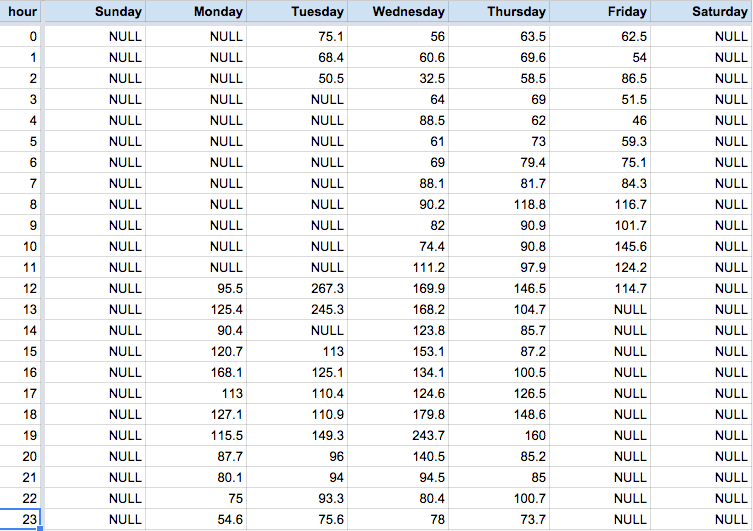
\includegraphics[width=0.9\textwidth]{figures/timetable_10002.png}
\caption{\label{fig:timetable_10002} Average journey time in seconds from stop 10002 to stop 11469 for each hour of each day of week}
\end{figure}

\par We plan to construct a timetable this way for each pair of the neighbouring bus stop.

\subsection{Filtering out the negative travel times}
\par In the travel\_time\_log generated, there were trips between two neighbouring stops with negative travel times, such as the entry shown in Table \ref{table:travel_time_log_negative}.

\begin{table}
\centering
\begin{tabular}{@{}lllllr@{}} \toprule
Start Stop & End Stop & Route & Start Time & End Time & Travel Time(sec) \\ \midrule
9326 & 15552 & W13 & 14:53:18 & 14:52:14 & -64 \\ \bottomrule
\end{tabular}
\caption{Travel Time Log Entry with Negative Travel Time}
\label{table:travel_time_log_negative}
\end{table}

\par This was because when we performed the join of the arrivals table, there was a more recent update on the arrival times for the start stop, whereas the arrival times of end stop had not been updated. In Table \ref{table:negative_travel_time_explained}, we observed that the Recorded Time for the end stop 9326 was more recent than that of the end stop. As a result, the arrival time for the end stop was earlier than the start stop, causing the travel time to be negative.

\begin{table}
\centering
\begin{tabular}{@{}lllllr@{}} \toprule
Stop Code & Route & Vehicle ID & Trip ID & Arrival Time & Recorded Time\\ \midrule
9326 & W13 & 18685 & 135229 &  14:53:18 & 14:48:25 \\ [0.4cm]
15552 & W13 & 18685 & 135229 & 14:52:14 & 14:44:02 \\ \bottomrule
\end{tabular}
\caption{Arrivals Entries to Explain Negative Travel Time}
\label{table:negative_travel_time_explained}
\end{table}

\par We filtered out these negative values before calculating the average travel time between neighbouring stops.

\section{Generating Reference Timetable}
\subsection{Journey Planner Bus Timetables}
\label{sec: official_tfl_timetable}
\todo[inline]{Need more detailed explanation. Walk through an example with xml code}
\par In order to calculate the delays in bus arrival times, we need the official bus travel times between stops for reference. This data was extracted from the Journey Planner Bus Timetables\cite{open_data_feeds_description} as part of the \acrshort{tfl} Open Data.


\par Each xml file contains bus schedule information for a route. For each day of the week, there are predefined number of VehicleJourneys running the give route throughout the day. We used the VehicleJourneys as a starting point to retrieve the departure time of the actual vehicle from the terminal. We then retrieve the corresponding JourneyPattern, and obtained the travel time between each neighbouring stops on the route for the given vehicle journey, to compute the cumulative travel times throughout the route.

The above computation was performed on each xml file to generate the actual arrival time and travel time for each vehicle trip at each stop in the route throughout the day. The results of this computation was stored in the delay\_tfl\_timetable table(Table \ref{table:delay_tfl_timetable}).

\begin{table}
\centering
\begin{tabular}{@{}llp{6cm}@{}} \toprule
Column Name & Type & Comments\\ \midrule
id(Primary Key) & int(11)  & Auto Increment\\ [0.4cm]
route & varchar(64) & The bus route \\ [0.4cm]
day & varchar(32) & The day of week for the vehicle journey \\ [0.4cm]
run & int(11) & The route direction \\ [0.4cm]
sequence & int (11) & The sequence of the bus stop in the route \\ [0.4cm]
stop\_name & varchar(64) & The name of the bus stop \\ [0.4cm]
naptan\_atco & varchar(64) & The national identifier of the bus stop \\ [0.4cm]
arrival\_time & datetime(6) & The expected arrival time for the given vehicle at the current bus stop \\ [0.4cm]
travel\_time & int(11) & The travel time in seconds from the previous stop in the route to the current stop \\ [0.4cm]
cumulative\_travel\_time & int(11) & The travel time  in seconds from the terminal to the current stop \\ [0.4cm]
departure\_time\_from\_origin & datetime(6) & The departure time of the given vehicle from the terminal \\
\bottomrule
\end{tabular}
\caption{delay\_tfl\_timetable Table Schema}
\label{table:delay_tfl_timetable}
\end{table}


%!TEX root = report.tex
\chapter{Serving the Data as REST API}

\section{Overview}
Objective of setting this up - to enable easy and fast query of the predictions I generated

\section{Frameworks}

\subsection{Django Framework}

\begin{itemize}
  \item what is it
  \item why did I choose it
  \item what are the available options and why do I choose the current one
\end{itemize}

\par Django is a high-level Python Web framework that encourages rapid development and clean, pragmatic design\cite{django_framework}.

\subsection{Django REST Framework}

\section{API Endpoints}
\begin{itemize}
  \item address of the endpoint
  \item parameters supplied
  \item return result format
\end{itemize}


\subsection{Historical \& Current}
\subsection{Reference}
\subsection{Arrival}



\section{Summary of data service}
Met the first objective by supplying data on bus travel time predictions

%!TEX root = report.tex
\chapter{Other Technical Details}


\section{Daemen Script Management - Supervisor}

\section{Scheduled Tasks Management - Jenkins}
\par We used Jenkins\cite{jenkins} to managed our predictions timetable update schedule.
\todo[inline]{add screenshots for jenkins}


\subsection{Current Timetable Update}
\par The current timetable is re-generated every hour. We set up a Jenkins job to re-run the relevant current timetable update SQL script every hour, and save the previous timetable into a log for updating the historical timetable at a later time. This job takes less than 10 minutes on average.

\subsection{Historical Timetable Update}
\par Similarly, we set up a Jenkins job to update the Historical Timetable daily at 3.30am when the server is less busy.

\subsection{Arrivals Daily Backup}
\par The arrivals table grows rapidly by approximately 150 thousand rows per hour. In order to allow fast access to the arrivals within the past one hour to construct the current timetable, we decided to save the arrivals for the current day in a new table, while keeping the past arrivals entries in an archive table. This required us to backup the arrivals entries daily to the arive.

\par Again, we created a Jenkins job to run the back up script daily. In order not to affect the historical timetable update, we set this job as a downstream task of the historical timetable update.

\subsection{Software Project Management - Trello}
\par We used Trello \cite{trello} for project management. It was useful to keep track of the tasks backlog, the tasks at hand, and the tasks to be further tested (Figure \ref{fig:trello}).

\begin{figure}
\centering
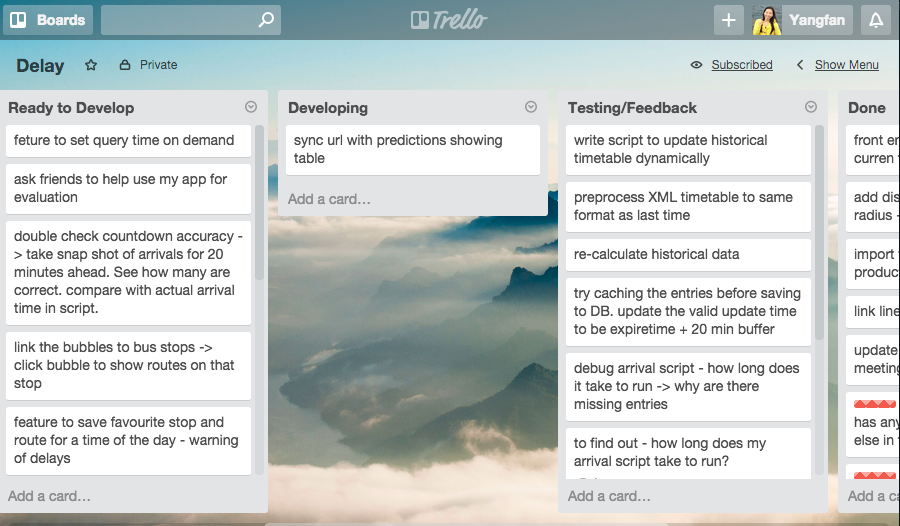
\includegraphics[width=\textwidth]{figures/trello_small.png}
\caption{\label{fig:trello} Project Trello Board}
\end{figure}

% %!TEX root = report.tex
\chapter{Project Plan}

\section{Project Objectives}
This project aims to produce a tool that notifies users of delays of the London buses they are waiting for, so that they can choose alternate routes and save waiting time.

\begin{description}
	\item[Back-end]  A timetable of bus journey times with an interface that supports real time query.
    \item[Front-end] A mobile application that allows users to check bus arrivals times with delay information at a give time and location.
\end{description}

\subsection{Core Features}
    \begin{enumerate}
        \item Given user current location, query for predicted bus arrivals at the nearest bus stop.
 		\item Give user current location and destination, query for routes and suggest bus routes with delays taken into consideration.
        \item Given starting location, destination, desired departure / arrival time, suggest bus routes with delays taken into consideration.
    \end{enumerate}

\subsection{Optional Extensions}
    \begin{enumerate}
    	\item Optimise prediction accuracy
        	\begin{itemize}
            	\item Analyse the average bus journey time for given starting and end stops to remove outliers.
                \item Integrate iBus actual arrivals data to improve arrivals timetable precision.
            \end{itemize}
        \item Include other modes of transportation for alternate route recommendation.
        \item Gather more user feedback on mobile application and improve accordingly .
        \item Publish mobile application on android market.
    \end{enumerate}

\section{Current Progress}
\begin{enumerate}
  \item Obtained access to TFL Live bus arrival API stream.
  \item Designed databases schema.
  \item Setup databases to store bus arrival data.
  \item Setup remote server to run daemon process to pull data from live bus arrivals feed and store data into the database.
  \item Collected 2 weeks of bus arrivals data for analysis.
  \item Created sample bus arrivals timetable for a chosen pair of neighbouring bus stops (10002 - 11469).
\end{enumerate}

\section{Development Plan}
\begin{description}
	\item \textbf{Spring Term Week 4}
    \begin{itemize}
    	\item Optimise arrivals table for fast query (e.g. via proper indexing).
		\item Create bus journey timetables with delay for all pairs of neighbouring bus stops.
    \end{itemize}
    \item \textbf{Spring Term Week 5}
    Develop journey planning feature with given start and end stops
    \item \textbf{Milestone 1 - Spring Term Week 6}
    Design query to request journey time from bus stop A to bus stop B at a given time of the day.

	\item \textbf{Spring Term Week 7}
    \begin{itemize}
    	\item Develop back-end API to receive query from mobile application.
    	\item Start initial mobile interface design.
    \end{itemize}
	\item \textbf{Spring Term Week 8}
	Design mobile application interface to extract user current location, and identify the nearest bus stop.
    \item \textbf{Milestone 2 - Spring Term Week 9}
    Connect mobile application to send query to the back-end to request for bus arrival times for all routes reaching ther nearest bus stop.
    \item \textbf{Spring Term Week 10}
    Improve mobile application user interface (gain user feedback and improve incrementally).
	\item \textbf{Fall-back Point - Easter Break}
    \begin{itemize}
    	\item Implement mobile interfaces to get journey destination for journey planning.
        \item Display suggested journey routes and travel time for a give time.
    	\item Optimise delay predictions by filtering out anomalies in average journey time calculation
    	\item Evaluate performance by comparing with iBus data
    \end{itemize}
    \item \textbf{Milestone 3 - Summer Term Week 1 - 3} Implement extensions and start writing report.
	\item \textbf{Summer Term Week 4} Report first draft.
    \item \textbf{Summer Term Week 5} Report second draft.
    \item \textbf{Summer Term Week 6} Presentation first draft.
    \item \textbf{Summer Term Week 7} Presentation second draft.
    \item \textbf{Summer Term Week 8}
    	\begin{itemize}
        	\item \textbf{Tuesday, 16th June 4pm} Final report due.
    		\item Presentation practice.
        \end{itemize}
    \item \textbf{Summer Term Week 9, Monday 22nd and Tuesday 23rd June} Presentation days.
    \item \textbf{Summer Term Week 10, Monday 29th June} Final Archive due.
\end{description}
%!TEX root = report.tex
\chapter{Evaluation}

\section{Compare predictions to real data}
We can compare the predictions generated to the live bus arrivals data stored in the arrivals table. We can calculate the standard deviation of the difference in the predicted time and actual arrival time. This value will be the direct indicator of the accuracy of the predictions.

\section{User feedback}
We can get students that take buses regularly to use the mobile application to test the accuracy of the delay predictions. The user feedback gathered will be the second input for evaluation.


\section{Accuracy}
How accurate are the predictions?


\section{Performance}
How reliable is the service?

\section{User feedback on UI}
How effective is it at warning delay?
>>>>>>> Stashed changes

% %!TEX root = report.tex

% %!TEX root = report.tex
\chapter{Future Work}
\par Future work for this project mainly involves the following 3 aspects.
\label{ch:future_work}
\begin{enumerate}
  \item \textbf{API Performance}
\par Currently, only one server is used for data collection, timetable generation, and live \acrshort{api} query handling. This could be the cause of the long response time. The performance of the API endpoints could be improved by using at least two servers, one in charge of data collection and processing, and the other handle live user queries. When the user base grow in the future, we could also setup more servers to process the requests concurrently.

\item \textbf{Prediction Accuracy}
\par The accuracy of the bus journey time predictions could be further tested and improved by applying more advanced analytical methods. These include but not limit to the approaches presented in the literature review (Section \ref{sec:literature}).
% refactor
% into separate components
% make it less tightly coupled
% data collection \& pre-processing
% server handling live user queries

\item \textbf{WebApp Extensions}
\par We could inclue features to alert users of bus delays actively for extension. The application should track the device location, and alert users of any delays occurred on the frequently travelled routes. The user interface could be furture improve the make the experience smoother. For example, a blue dot could be added to the map to indicate the current location of the device, and be updated constantly. Additionally, bus journey planning and the ability to search start and end stops are also helpful.
\end{enumerate}



% %!TEX root = report.tex
\chapter{Conclusion}

\par In this project, we built a data service to provide the average bus travel time for each downstream stop for a given route on a given day of the week and hour of the day. This prediction data API can support about 100 simultaneous users.

\par We also designed a demonstrative web application to showcase the potential use of the data service.



\cleardoublepage
%\pagebreak
\phantomsection
\addcontentsline{toc}{chapter}{References}
\begin{thebibliography}{99}

\bibitem{tfl_annual_report_13/14} Transport for London Annual Report and Statement of Accounts 2013/14, \
\url{http://tfl.gov.uk/cdn/static/cms/documents/annual-report-2013-14.pdf} [visited on 27/01/2015]

\bibitem{live_bus_arrivals} Transport for London Live Bus Arrivals, \
\url{http://www.tfl.gov.uk/modes/buses/live-bus-arrivals} [visited on 27/01/2015]

\bibitem{google_maps} Google Maps, \
\url{https://www.google.co.uk/maps} [visited on 30/01/2015]

\bibitem{citymapper} CityMapper, \
\url{https://citymapper.com/london} [visited on 30/01/2015]

\bibitem{tfl_journey_planner} TfL Plan A Journey, \
\url{http://tfl.gov.uk/plan-a-journey/} [visited on 30/01/2015]

\bibitem{buses_performance_report} Transport for London Buses Network Performance Second Quarter 2014/15, \
\url{http://tfl.gov.uk/cdn/static/cms/documents/network-performance-latest-quarter.pdf} [visited on 27/01/2015]

\bibitem{tfl_ltds} Travel in London, Supplementary Report: London Travel Demand Survey (LTDS), \
\url{http://www.tfl.gov.uk/cdn/static/cms/documents/london-travel-demand-survey.pdf} [visited on 28/01/2015]

\bibitem{bus_stop_locations_routes} Transport for London Bus Stops Locations and Routes Open Data\
\url{https://www.tfl.gov.uk/info-for/open-data-users/our-feeds} [visited on 28/01/2015]

\bibitem{open_data} Transport for London Open Data\
\url{https://www.tfl.gov.uk/info-for/open-data-users/our-open-data} [visited on 28/01/2015]

\bibitem{live_bus_api_documentation} Transport for London Live Bus \& River Bus Arrivals API Interface Documentation\
\url{https://www.tfl.gov.uk/cdn/static/cms/documents/tfl-live-bus-river-bus-arrivals-api-documentation-v16.pdf} [visited on 28/01/2015]

\bibitem{buses_performance_data} Transport for London Buses Performance Data\
\url{https://www.tfl.gov.uk/corporate/publications-and-reports/buses-performance-data#on-this-page-5} [visited on 28/01/2015]

\end{thebibliography}

\end{document}